%%%%%%%%%%%%%%%%%%%%%%%%%%%%%%%%%%%%%%%%
% original template
%%%%%%%%%%%%%%%%%%%%%%%%%%%%%%%%%%%%%%%%

\documentclass[10pt,twocolumn,letterpaper]{article}

\usepackage{cvpr}
\usepackage{multirow}
%%%%% NEW MATH DEFINITIONS %%%%%

\usepackage{amsmath,amsfonts,bm}

% Mark sections of captions for referring to divisions of figures
\newcommand{\figleft}{{\em (Left)}}
\newcommand{\figcenter}{{\em (Center)}}
\newcommand{\figright}{{\em (Right)}}
\newcommand{\figtop}{{\em (Top)}}
\newcommand{\figbottom}{{\em (Bottom)}}
\newcommand{\captiona}{{\em (a)}}
\newcommand{\captionb}{{\em (b)}}
\newcommand{\captionc}{{\em (c)}}
\newcommand{\captiond}{{\em (d)}}

% Highlight a newly defined term
\newcommand{\newterm}[1]{{\bf #1}}


% Figure reference, lower-case.
\def\figref#1{figure~\ref{#1}}
% Figure reference, capital. For start of sentence
\def\Figref#1{Figure~\ref{#1}}
\def\twofigref#1#2{figures \ref{#1} and \ref{#2}}
\def\quadfigref#1#2#3#4{figures \ref{#1}, \ref{#2}, \ref{#3} and \ref{#4}}
% Section reference, lower-case.
\def\secref#1{section~\ref{#1}}
% Section reference, capital.
\def\Secref#1{Section~\ref{#1}}
% Reference to two sections.
\def\twosecrefs#1#2{sections \ref{#1} and \ref{#2}}
% Reference to three sections.
\def\secrefs#1#2#3{sections \ref{#1}, \ref{#2} and \ref{#3}}
% Reference to an equation, lower-case.
\def\eqref#1{equation~\ref{#1}}
% Reference to an equation, upper case
\def\Eqref#1{Equation~\ref{#1}}
% A raw reference to an equation---avoid using if possible
\def\plaineqref#1{\ref{#1}}
% Reference to a chapter, lower-case.
\def\chapref#1{chapter~\ref{#1}}
% Reference to an equation, upper case.
\def\Chapref#1{Chapter~\ref{#1}}
% Reference to a range of chapters
\def\rangechapref#1#2{chapters\ref{#1}--\ref{#2}}
% Reference to an algorithm, lower-case.
\def\algref#1{algorithm~\ref{#1}}
% Reference to an algorithm, upper case.
\def\Algref#1{Algorithm~\ref{#1}}
\def\twoalgref#1#2{algorithms \ref{#1} and \ref{#2}}
\def\Twoalgref#1#2{Algorithms \ref{#1} and \ref{#2}}
% Reference to a part, lower case
\def\partref#1{part~\ref{#1}}
% Reference to a part, upper case
\def\Partref#1{Part~\ref{#1}}
\def\twopartref#1#2{parts \ref{#1} and \ref{#2}}

\def\ceil#1{\lceil #1 \rceil}
\def\floor#1{\lfloor #1 \rfloor}
\def\1{\bm{1}}
\newcommand{\train}{\mathcal{D}}
\newcommand{\valid}{\mathcal{D_{\mathrm{valid}}}}
\newcommand{\test}{\mathcal{D_{\mathrm{test}}}}

\def\eps{{\epsilon}}


% Random variables
\def\reta{{\textnormal{$\eta$}}}
\def\ra{{\textnormal{a}}}
\def\rb{{\textnormal{b}}}
\def\rc{{\textnormal{c}}}
\def\rd{{\textnormal{d}}}
\def\re{{\textnormal{e}}}
\def\rf{{\textnormal{f}}}
\def\rg{{\textnormal{g}}}
\def\rh{{\textnormal{h}}}
\def\ri{{\textnormal{i}}}
\def\rj{{\textnormal{j}}}
\def\rk{{\textnormal{k}}}
\def\rl{{\textnormal{l}}}
% rm is already a command, just don't name any random variables m
\def\rn{{\textnormal{n}}}
\def\ro{{\textnormal{o}}}
\def\rp{{\textnormal{p}}}
\def\rq{{\textnormal{q}}}
\def\rr{{\textnormal{r}}}
\def\rs{{\textnormal{s}}}
\def\rt{{\textnormal{t}}}
\def\ru{{\textnormal{u}}}
\def\rv{{\textnormal{v}}}
\def\rw{{\textnormal{w}}}
\def\rx{{\textnormal{x}}}
\def\ry{{\textnormal{y}}}
\def\rz{{\textnormal{z}}}

% Random vectors
\def\rvepsilon{{\mathbf{\epsilon}}}
\def\rvtheta{{\mathbf{\theta}}}
\def\rva{{\mathbf{a}}}
\def\rvb{{\mathbf{b}}}
\def\rvc{{\mathbf{c}}}
\def\rvd{{\mathbf{d}}}
\def\rve{{\mathbf{e}}}
\def\rvf{{\mathbf{f}}}
\def\rvg{{\mathbf{g}}}
\def\rvh{{\mathbf{h}}}
\def\rvu{{\mathbf{i}}}
\def\rvj{{\mathbf{j}}}
\def\rvk{{\mathbf{k}}}
\def\rvl{{\mathbf{l}}}
\def\rvm{{\mathbf{m}}}
\def\rvn{{\mathbf{n}}}
\def\rvo{{\mathbf{o}}}
\def\rvp{{\mathbf{p}}}
\def\rvq{{\mathbf{q}}}
\def\rvr{{\mathbf{r}}}
\def\rvs{{\mathbf{s}}}
\def\rvt{{\mathbf{t}}}
\def\rvu{{\mathbf{u}}}
\def\rvv{{\mathbf{v}}}
\def\rvw{{\mathbf{w}}}
\def\rvx{{\mathbf{x}}}
\def\rvy{{\mathbf{y}}}
\def\rvz{{\mathbf{z}}}

% Elements of random vectors
\def\erva{{\textnormal{a}}}
\def\ervb{{\textnormal{b}}}
\def\ervc{{\textnormal{c}}}
\def\ervd{{\textnormal{d}}}
\def\erve{{\textnormal{e}}}
\def\ervf{{\textnormal{f}}}
\def\ervg{{\textnormal{g}}}
\def\ervh{{\textnormal{h}}}
\def\ervi{{\textnormal{i}}}
\def\ervj{{\textnormal{j}}}
\def\ervk{{\textnormal{k}}}
\def\ervl{{\textnormal{l}}}
\def\ervm{{\textnormal{m}}}
\def\ervn{{\textnormal{n}}}
\def\ervo{{\textnormal{o}}}
\def\ervp{{\textnormal{p}}}
\def\ervq{{\textnormal{q}}}
\def\ervr{{\textnormal{r}}}
\def\ervs{{\textnormal{s}}}
\def\ervt{{\textnormal{t}}}
\def\ervu{{\textnormal{u}}}
\def\ervv{{\textnormal{v}}}
\def\ervw{{\textnormal{w}}}
\def\ervx{{\textnormal{x}}}
\def\ervy{{\textnormal{y}}}
\def\ervz{{\textnormal{z}}}

% Random matrices
\def\rmA{{\mathbf{A}}}
\def\rmB{{\mathbf{B}}}
\def\rmC{{\mathbf{C}}}
\def\rmD{{\mathbf{D}}}
\def\rmE{{\mathbf{E}}}
\def\rmF{{\mathbf{F}}}
\def\rmG{{\mathbf{G}}}
\def\rmH{{\mathbf{H}}}
\def\rmI{{\mathbf{I}}}
\def\rmJ{{\mathbf{J}}}
\def\rmK{{\mathbf{K}}}
\def\rmL{{\mathbf{L}}}
\def\rmM{{\mathbf{M}}}
\def\rmN{{\mathbf{N}}}
\def\rmO{{\mathbf{O}}}
\def\rmP{{\mathbf{P}}}
\def\rmQ{{\mathbf{Q}}}
\def\rmR{{\mathbf{R}}}
\def\rmS{{\mathbf{S}}}
\def\rmT{{\mathbf{T}}}
\def\rmU{{\mathbf{U}}}
\def\rmV{{\mathbf{V}}}
\def\rmW{{\mathbf{W}}}
\def\rmX{{\mathbf{X}}}
\def\rmY{{\mathbf{Y}}}
\def\rmZ{{\mathbf{Z}}}

% Elements of random matrices
\def\ermA{{\textnormal{A}}}
\def\ermB{{\textnormal{B}}}
\def\ermC{{\textnormal{C}}}
\def\ermD{{\textnormal{D}}}
\def\ermE{{\textnormal{E}}}
\def\ermF{{\textnormal{F}}}
\def\ermG{{\textnormal{G}}}
\def\ermH{{\textnormal{H}}}
\def\ermI{{\textnormal{I}}}
\def\ermJ{{\textnormal{J}}}
\def\ermK{{\textnormal{K}}}
\def\ermL{{\textnormal{L}}}
\def\ermM{{\textnormal{M}}}
\def\ermN{{\textnormal{N}}}
\def\ermO{{\textnormal{O}}}
\def\ermP{{\textnormal{P}}}
\def\ermQ{{\textnormal{Q}}}
\def\ermR{{\textnormal{R}}}
\def\ermS{{\textnormal{S}}}
\def\ermT{{\textnormal{T}}}
\def\ermU{{\textnormal{U}}}
\def\ermV{{\textnormal{V}}}
\def\ermW{{\textnormal{W}}}
\def\ermX{{\textnormal{X}}}
\def\ermY{{\textnormal{Y}}}
\def\ermZ{{\textnormal{Z}}}

% Vectors
\def\vzero{{\bm{0}}}
\def\vone{{\bm{1}}}
\def\vmu{{\bm{\mu}}}
\def\vtheta{{\bm{\theta}}}
\def\va{{\bm{a}}}
\def\vb{{\bm{b}}}
\def\vc{{\bm{c}}}
\def\vd{{\bm{d}}}
\def\ve{{\bm{e}}}
\def\vf{{\bm{f}}}
\def\vg{{\bm{g}}}
\def\vh{{\bm{h}}}
\def\vi{{\bm{i}}}
\def\vj{{\bm{j}}}
\def\vk{{\bm{k}}}
\def\vl{{\bm{l}}}
\def\vm{{\bm{m}}}
\def\vn{{\bm{n}}}
\def\vo{{\bm{o}}}
\def\vp{{\bm{p}}}
\def\vq{{\bm{q}}}
\def\vr{{\bm{r}}}
\def\vs{{\bm{s}}}
\def\vt{{\bm{t}}}
\def\vu{{\bm{u}}}
\def\vv{{\bm{v}}}
\def\vw{{\bm{w}}}
\def\vx{{\bm{x}}}
\def\vy{{\bm{y}}}
\def\vz{{\bm{z}}}

% Elements of vectors
\def\evalpha{{\alpha}}
\def\evbeta{{\beta}}
\def\evepsilon{{\epsilon}}
\def\evlambda{{\lambda}}
\def\evomega{{\omega}}
\def\evmu{{\mu}}
\def\evpsi{{\psi}}
\def\evsigma{{\sigma}}
\def\evtheta{{\theta}}
\def\eva{{a}}
\def\evb{{b}}
\def\evc{{c}}
\def\evd{{d}}
\def\eve{{e}}
\def\evf{{f}}
\def\evg{{g}}
\def\evh{{h}}
\def\evi{{i}}
\def\evj{{j}}
\def\evk{{k}}
\def\evl{{l}}
\def\evm{{m}}
\def\evn{{n}}
\def\evo{{o}}
\def\evp{{p}}
\def\evq{{q}}
\def\evr{{r}}
\def\evs{{s}}
\def\evt{{t}}
\def\evu{{u}}
\def\evv{{v}}
\def\evw{{w}}
\def\evx{{x}}
\def\evy{{y}}
\def\evz{{z}}

% Matrix
\def\mA{{\bm{A}}}
\def\mB{{\bm{B}}}
\def\mC{{\bm{C}}}
\def\mD{{\bm{D}}}
\def\mE{{\bm{E}}}
\def\mF{{\bm{F}}}
\def\mG{{\bm{G}}}
\def\mH{{\bm{H}}}
\def\mI{{\bm{I}}}
\def\mJ{{\bm{J}}}
\def\mK{{\bm{K}}}
\def\mL{{\bm{L}}}
\def\mM{{\bm{M}}}
\def\mN{{\bm{N}}}
\def\mO{{\bm{O}}}
\def\mP{{\bm{P}}}
\def\mQ{{\bm{Q}}}
\def\mR{{\bm{R}}}
\def\mS{{\bm{S}}}
\def\mT{{\bm{T}}}
\def\mU{{\bm{U}}}
\def\mV{{\bm{V}}}
\def\mW{{\bm{W}}}
\def\mX{{\bm{X}}}
\def\mY{{\bm{Y}}}
\def\mZ{{\bm{Z}}}
\def\mBeta{{\bm{\beta}}}
\def\mPhi{{\bm{\Phi}}}
\def\mLambda{{\bm{\Lambda}}}
\def\mSigma{{\bm{\Sigma}}}

% Tensor
\DeclareMathAlphabet{\mathsfit}{\encodingdefault}{\sfdefault}{m}{sl}
\SetMathAlphabet{\mathsfit}{bold}{\encodingdefault}{\sfdefault}{bx}{n}
\newcommand{\tens}[1]{\bm{\mathsfit{#1}}}
\def\tA{{\tens{A}}}
\def\tB{{\tens{B}}}
\def\tC{{\tens{C}}}
\def\tD{{\tens{D}}}
\def\tE{{\tens{E}}}
\def\tF{{\tens{F}}}
\def\tG{{\tens{G}}}
\def\tH{{\tens{H}}}
\def\tI{{\tens{I}}}
\def\tJ{{\tens{J}}}
\def\tK{{\tens{K}}}
\def\tL{{\tens{L}}}
\def\tM{{\tens{M}}}
\def\tN{{\tens{N}}}
\def\tO{{\tens{O}}}
\def\tP{{\tens{P}}}
\def\tQ{{\tens{Q}}}
\def\tR{{\tens{R}}}
\def\tS{{\tens{S}}}
\def\tT{{\tens{T}}}
\def\tU{{\tens{U}}}
\def\tV{{\tens{V}}}
\def\tW{{\tens{W}}}
\def\tX{{\tens{X}}}
\def\tY{{\tens{Y}}}
\def\tZ{{\tens{Z}}}


% Graph
\def\gA{{\mathcal{A}}}
\def\gB{{\mathcal{B}}}
\def\gC{{\mathcal{C}}}
\def\gD{{\mathcal{D}}}
\def\gE{{\mathcal{E}}}
\def\gF{{\mathcal{F}}}
\def\gG{{\mathcal{G}}}
\def\gH{{\mathcal{H}}}
\def\gI{{\mathcal{I}}}
\def\gJ{{\mathcal{J}}}
\def\gK{{\mathcal{K}}}
\def\gL{{\mathcal{L}}}
\def\gM{{\mathcal{M}}}
\def\gN{{\mathcal{N}}}
\def\gO{{\mathcal{O}}}
\def\gP{{\mathcal{P}}}
\def\gQ{{\mathcal{Q}}}
\def\gR{{\mathcal{R}}}
\def\gS{{\mathcal{S}}}
\def\gT{{\mathcal{T}}}
\def\gU{{\mathcal{U}}}
\def\gV{{\mathcal{V}}}
\def\gW{{\mathcal{W}}}
\def\gX{{\mathcal{X}}}
\def\gY{{\mathcal{Y}}}
\def\gZ{{\mathcal{Z}}}

% Sets
\def\sA{{\mathbb{A}}}
\def\sB{{\mathbb{B}}}
\def\sC{{\mathbb{C}}}
\def\sD{{\mathbb{D}}}
% Don't use a set called E, because this would be the same as our symbol
% for expectation.
\def\sF{{\mathbb{F}}}
\def\sG{{\mathbb{G}}}
\def\sH{{\mathbb{H}}}
\def\sI{{\mathbb{I}}}
\def\sJ{{\mathbb{J}}}
\def\sK{{\mathbb{K}}}
\def\sL{{\mathbb{L}}}
\def\sM{{\mathbb{M}}}
\def\sN{{\mathbb{N}}}
\def\sO{{\mathbb{O}}}
\def\sP{{\mathbb{P}}}
\def\sQ{{\mathbb{Q}}}
\def\sR{{\mathbb{R}}}
\def\sS{{\mathbb{S}}}
\def\sT{{\mathbb{T}}}
\def\sU{{\mathbb{U}}}
\def\sV{{\mathbb{V}}}
\def\sW{{\mathbb{W}}}
\def\sX{{\mathbb{X}}}
\def\sY{{\mathbb{Y}}}
\def\sZ{{\mathbb{Z}}}

% Entries of a matrix
\def\emLambda{{\Lambda}}
\def\emA{{A}}
\def\emB{{B}}
\def\emC{{C}}
\def\emD{{D}}
\def\emE{{E}}
\def\emF{{F}}
\def\emG{{G}}
\def\emH{{H}}
\def\emI{{I}}
\def\emJ{{J}}
\def\emK{{K}}
\def\emL{{L}}
\def\emM{{M}}
\def\emN{{N}}
\def\emO{{O}}
\def\emP{{P}}
\def\emQ{{Q}}
\def\emR{{R}}
\def\emS{{S}}
\def\emT{{T}}
\def\emU{{U}}
\def\emV{{V}}
\def\emW{{W}}
\def\emX{{X}}
\def\emY{{Y}}
\def\emZ{{Z}}
\def\emSigma{{\Sigma}}

% entries of a tensor
% Same font as tensor, without \bm wrapper
\newcommand{\etens}[1]{\mathsfit{#1}}
\def\etLambda{{\etens{\Lambda}}}
\def\etA{{\etens{A}}}
\def\etB{{\etens{B}}}
\def\etC{{\etens{C}}}
\def\etD{{\etens{D}}}
\def\etE{{\etens{E}}}
\def\etF{{\etens{F}}}
\def\etG{{\etens{G}}}
\def\etH{{\etens{H}}}
\def\etI{{\etens{I}}}
\def\etJ{{\etens{J}}}
\def\etK{{\etens{K}}}
\def\etL{{\etens{L}}}
\def\etM{{\etens{M}}}
\def\etN{{\etens{N}}}
\def\etO{{\etens{O}}}
\def\etP{{\etens{P}}}
\def\etQ{{\etens{Q}}}
\def\etR{{\etens{R}}}
\def\etS{{\etens{S}}}
\def\etT{{\etens{T}}}
\def\etU{{\etens{U}}}
\def\etV{{\etens{V}}}
\def\etW{{\etens{W}}}
\def\etX{{\etens{X}}}
\def\etY{{\etens{Y}}}
\def\etZ{{\etens{Z}}}

% The true underlying data generating distribution
\newcommand{\pdata}{p_{\rm{data}}}
% The empirical distribution defined by the training set
\newcommand{\ptrain}{\hat{p}_{\rm{data}}}
\newcommand{\Ptrain}{\hat{P}_{\rm{data}}}
% The model distribution
\newcommand{\pmodel}{p_{\rm{model}}}
\newcommand{\Pmodel}{P_{\rm{model}}}
\newcommand{\ptildemodel}{\tilde{p}_{\rm{model}}}
% Stochastic autoencoder distributions
\newcommand{\pencode}{p_{\rm{encoder}}}
\newcommand{\pdecode}{p_{\rm{decoder}}}
\newcommand{\precons}{p_{\rm{reconstruct}}}

\newcommand{\laplace}{\mathrm{Laplace}} % Laplace distribution

\newcommand{\E}{\mathbb{E}}
\newcommand{\Ls}{\mathcal{L}}
\newcommand{\R}{\mathbb{R}}
\newcommand{\emp}{\tilde{p}}
\newcommand{\lr}{\alpha}
\newcommand{\reg}{\lambda}
\newcommand{\rect}{\mathrm{rectifier}}
\newcommand{\softmax}{\mathrm{softmax}}
\newcommand{\sigmoid}{\sigma}
\newcommand{\softplus}{\zeta}
\newcommand{\KL}{D_{\mathrm{KL}}}
\newcommand{\Var}{\mathrm{Var}}
\newcommand{\standarderror}{\mathrm{SE}}
\newcommand{\Cov}{\mathrm{Cov}}
% Wolfram Mathworld says $L^2$ is for function spaces and $\ell^2$ is for vectors
% But then they seem to use $L^2$ for vectors throughout the site, and so does
% wikipedia.
\newcommand{\normlzero}{L^0}
\newcommand{\normlone}{L^1}
\newcommand{\normltwo}{L^2}
\newcommand{\normlp}{L^p}
\newcommand{\normmax}{L^\infty}

\newcommand{\parents}{Pa} % See usage in notation.tex. Chosen to match Daphne's book.

\DeclareMathOperator*{\argmax}{arg\,max}
\DeclareMathOperator*{\argmin}{arg\,min}

\DeclareMathOperator{\sign}{sign}
\DeclareMathOperator{\Tr}{Tr}
\let\ab\allowbreak

\usepackage{times}
\usepackage{epsfig}
\usepackage{graphicx}
\usepackage[]{algorithm2e}
\usepackage{amsthm}
\usepackage{mathrsfs}
\usepackage{amsmath, amssymb}
\usepackage[numbers,sort&compress]{natbib}  % 自动将[1,2,3]转为[1-3]

% Include other packages here, before hyperref.

% If you comment hyperref and then uncomment it, you should delete
% egpaper.aux before re-running latex.  (Or just hit 'q' on the first latex
% run, let it finish, and you should be clear).
\usepackage[pagebackref=true,breaklinks=true,letterpaper=true,colorlinks,bookmarks=false]{hyperref}

% todo:
% \cvprfinalcopy % *** Uncomment this line for the final submission

\def\cvprPaperID{xxxx} % *** Enter the CVPR Paper ID here
\def\httilde{\mbox{\tt\raisebox{-.5ex}{\symbol{126}}}}

% Pages are numbered in submission mode, and unnumbered in camera-ready
\ifcvprfinal\pagestyle{empty}\fi

%%%%%%%%%%%%%%%%%%%%%%%%%%%%%%%%%%%%%%%%
% micla
%%%%%%%%%%%%%%%%%%%%%%%%%%%%%%%%%%%%%%%%

% abbreviations
\usepackage{xspace}
\newcommand{\DCCK}{BSConv\xspace}
\newcommand{\DCCKU}{\DCCK-U\xspace}
\newcommand{\DCCKS}{\DCCK-S\xspace}

% refs
\usepackage{cleveref}

% latin abbreviations
\renewcommand{\cf}{\textit{cf.\@\xspace}}

% ?
% \newcommand*{\vcenteredhbox}[1]{\begingroup
% \setbox0=\hbox{#1}\parbox{\wd0}{\box0}\endgroup}
% \usepackage{adjustbox}
% \newcommand{\vcenteredhbox}[1]{\adjustbox{valign=c}{#1}}
% \adjustbox{valign=c}{文本} % 直接使用 

% todo command
\usepackage{xcolor}
\newcommand{\todo}[1]{\textcolor{red}{#1}}

% insert one column worth of empty lines...
\newcommand{\emptycol}{\vspace*{\fill}}

% used symbols
\usepackage{amssymb}
\newcommand{\tensorIn}{U}
\newcommand{\tensorOut}{V}
\newcommand{\filter}[1]{F^{(#1)}}
\newcommand{\blueprint}[1]{B^{(#1)}}
\newcommand{\blueprintWidthwise}{B'}
\newcommand{\weight}{w}
\newcommand{\weightArray}{\tilde{w}}
\newcommand{\weightA}{w^A}
\newcommand{\weightAArray}{\tilde{w}^A}
\newcommand{\weightB}{w^B}
\newcommand{\weightBArray}{\tilde{w}^B}
\newcommand{\weightMatrix}{W}
\newcommand{\weightMatrixA}{W^A}
\newcommand{\weightMatrixB}{W^B}
\newcommand{\spatialV}{Y}
\newcommand{\spatialW}{X}
\newcommand{\spatialK}{K}
\newcommand{\spatialKIndex}{k}
\newcommand{\channelInCount}{M}
\newcommand{\channelInIndex}{m}
\newcommand{\channelOutCount}{N}
\newcommand{\channelOutIndex}{n}

% better page layout
\clubpenalty = 1
\widowpenalty = 1
\displaywidowpenalty = 1

% used for width factors such as `(x0.75)'
\newcommand{\widthFactor}[1]{(x#1)}

%%%%%%%%%%%%%%%%%%%%%%%%%%%%%%%%%%%%%%%%
% document
%%%%%%%%%%%%%%%%%%%%%%%%%%%%%%%%%%%%%%%%

\begin{document}

% space optimization (less space between text and equations)
\setlength{\abovedisplayskip}{5pt}
\setlength{\belowdisplayskip}{5pt}
\setlength{\abovedisplayskip}{5pt}
\setlength{\belowdisplayskip}{5pt}

%%%%%%%%%%%%%%%%%%%%%%%%%%%%%%%%%%%%%%%%
% frontmatter
%%%%%%%%%%%%%%%%%%%%%%%%%%%%%%%%%%%%%%%%

\title{When and How Much to Perturb? Decoding Radius-Timing-Scale(RTS) in PUGD Optimization}

\author{Zongyuan Sui\\
Independent researcher\\
{\tt\small 15763036963@163.com}
}

\maketitle
\thispagestyle{empty}

%%%%%%%%%%%%%%%%%%%%%%%%%%%%%%%%%%%%%%%%
% abstract
%%%%%%%%%%%%%%%%%%%%%%%%%%%%%%%%%%%%%%%%
% \todo: add github,change data, finish this part
\begin{abstract} 8-10lines
We demonstrate 'Radius-Timing-Scale(RTS)' as algorithmic enhancements to the \textit{Perturbated Unit Gradient Descent (PUGD)}.
Optimization algorithms are pivotal in deep learning, particularly for image classification tasks. \textit{Perturbated Unit Gradient Descent (PUGD)} \cite{Tseng_2022} introduces a novel update rule with limitations of high computational costs that cant reach the better Top-1 accuracy when compared with benchmark SGD when SGD reached convergence. 

This work tries to alleviate such gap by investigating the limitations of Perturbated Unit Gradient Descent (PUGD) optimizer, proposing a novel additional parameter tuning strategy that adjusts both the perturbation radius, timing of using it and the scale of gradient. It is analogous to learning rate scheduling, systematic adjustment of perturbation radius and scale of gradient boosts PUGD's performance.Meanwhile, our proposed approaches addressed the question—within a limited scope—of whether perturbation radius and gradient scale should be large or small during different training phases. Code and results are available under \url{https://github.com/eeyzs1}.
\end{abstract}
\vspace{-1.25em}

%%%%%%%%%%%%%%%%%%%%%%%%%%%%%%%%%%%%%%%%
% introduction
%%%%%%%%%%%%%%%%%%%%%%%%%%%%%%%%%%%%%%%%
\section{Introduction} 40lines+fig/1page
Stochastic Gradient Descent (SGD) \cite{4308316} remains a cornerstone for iterative model optimization, yet it faces one limitation: While theoretical analysis in Kawaguchi' study \cite{kawaguchi2016deeplearningpoorlocal} demonstrates that deep learning models rarely become trapped in strict saddle points or local minima, empirical evidence shows performance variance across different model architectures and training protocols for different tasks. In other word, sharp minima hinder generalization, as shown in the work from Foret et al.\cite{foret2021sharpnessawareminimizationefficientlyimproving}, causing poor performance on new scenarios. These challenges have spurred numerous algorithmic variants, each aiming to mitigate specific drawbacks of vanilla GD \cite{ruder2017overviewgradientdescentoptimization}.

The \textit{Perturbated Unit Gradient Descent (PUGD)} \cite{Tseng_2022} introduces a novel update rule: gradient perturbation with unit normalization by scaling the combined (original + perturbed) gradient with unit dual norm, which ensures stable updates. This algorithm addresses generalization improvement and saddle point mitigation simultaneously.

\begin{figure}[htbp]
	\center
	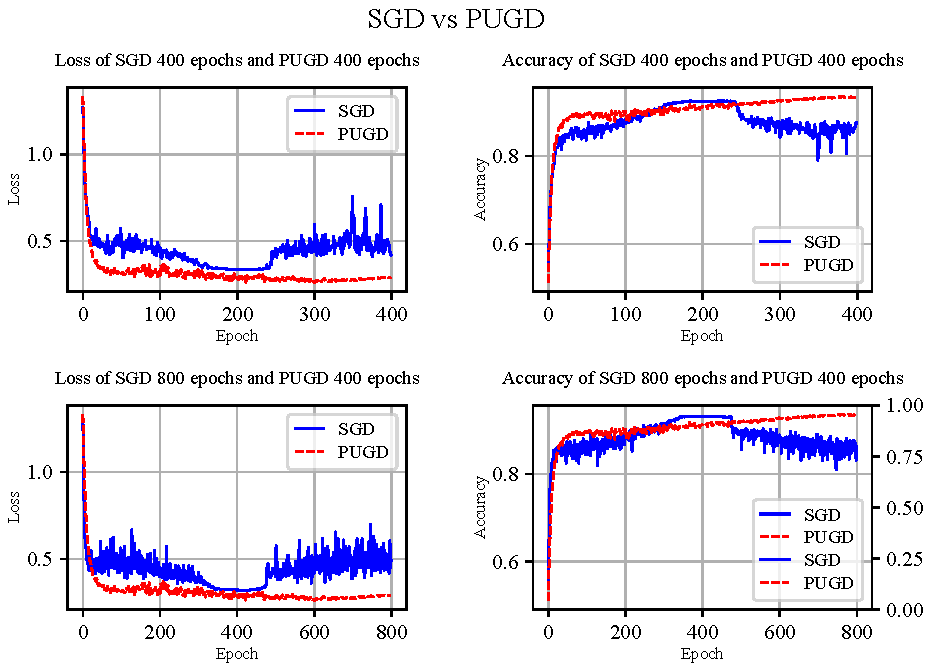
\includegraphics[width=\columnwidth]{images/SGDvsPUGD.pdf}
	\caption{Training histories of SGD and PUGD
    \textbf{Top row}: Loss and accuracy of both optimizers (400 epochs)
    \textbf{Bottom row}: SGD (800 epochs) vs PUGD (400 epochs)}
	\label{fig:SGDvsPUGD}
\end{figure}

Although Tseng et al. \cite{Tseng_2022} reported that PUGD outperformed \textit{Stochastic Gradient Descent (SGD)} \cite{4308316} under matched epoch budgets, my CIFAR-10 experiments (\Cref{fig:SGDvsPUGD}) reveal a divergence: PUGD fails to match SGD's convergence speed in early training phases, though it eventually achieves higher peak accuracy after extended optimization. This suggests a trade-off between initial convergence rate and final performance, which means potential optimization possibilities.
Inspired by this finding and \textit{cosine annealing} \cite{loshchilov2017sgdrstochasticgradientdescent}, which is a learning rate scheduling technique that dynamically adjusts the learning rate ($eta_t$) during training following a cosine-shaped decay curve. Mathematically, it is defined as: $\eta_t = \eta_{\min} + \frac{1}{2}(\eta_{\max} - \eta_{\min})\left(1 + \cos\left(\frac{T_{\text{cur}}}{T_{\max}}\pi\right)\right)$. Therefore we want to propose enhancements from three aspects: 1. An adapted perturbation scheduler for PUGD that dynamically adjusts the exploration radius through cyclical temperature decay, enabling phase-wise trade-offs between exploration and exploitation. 2. An adaptive SGD-PUGD hybrid that leverages SGD's rapid initial convergence in early training stages, then transitions to PUGD's perturbation-based refinement for sharpness-aware generalization, achieving both training efficiency and flat-minima convergence. 3. Tunning the scale of gradient so that influence the gradient descent direction reasonablely. The integration of these three enhancements is formally designated as 'Radius-Timing Scale(RTS)'.
In brief, the main contributions in this work include: 
\begin{enumerate}
    \item[(1)] Perturbation Radius Tuning: Analogous to cosine annealing learning rate scheduling, the systematic adjustment of perturbation radiuss boosts PUGD performance.
    \item[(2)] Computational Efficiency: PUGD is applied efficiently at an appropriate time rather than at the beginning of training. 
    \item[(3)] Scale of gradient Tunning: the systematic adjustment of gradient boosts PUGD performance.
    \item[(4)] The tuning coefficient $\alpha$: four adaptive update strategies.
    \item[(5)] Integrated Solution: Combining perturbation radius and timing control yields synergistic effects and demonstrates the complete optimization process. 
    \item[(6)] Results comparisons: The results compare the proposed method with PUGD and SGD, showing improvements from Radius-Timing Scale(RTS). 
\end{enumerate}
This paper is divided into five parts. First, the background, motivation and a summary of Radius-Timing Scale(RTS) have been present in this. Then, in \Cref{sec:2}, the mechanism and its limitations. After, we present the explanation of Radius-Timing Scale(RTS) enhancement in \Cref{sec:3}. Finally, a series of experiments on PUGD and enhancement is shown in \Cref{sec:4}, with the conclusion in \Cref{sec:5} and supplements in Appendix. 
%%%%%%%%%%%%%%%%%%%%%%%%%%%%%%%%%%%%%%%%
% related work
%%%%%%%%%%%%%%%%%%%%%%%%%%%%%%%%%%%%%%%%

\section{Related Work}
\label{sec:2}
Since Stochastic Gradient Descent (SGD) \cite{4308316} first emerged as an optimization technique, it has gradually become the de facto standard optimizer across machine learning paradigms, owing to its computational efficiency and proven empirical success in large-scale learning scenarios.
Whereas modern neural networks exhibit complex, non-convex loss landscapes with multiple global minima that demonstrate distinct generalization capabilities \cite{keskar2017largebatchtrainingdeeplearning}. With the theoretical support from \cite{ji2020directionalconvergencealignmentdeep} that the local Lipschitz condition ensures gradient flow(infinitesimal gradient descent) trajectories avoid oscillatory paths, while SGD noise helps escape sharp basins-jointly contributing to the flat minima. As well as Empirical evidence suggests that gradient normalization can enhance generalization, as demonstrated in prior work. For instance, Path-SGD \cite{neyshabur2015pathsgdpathnormalizedoptimizationdeep} employs path-normalized updates to improve optimization in deep networks, while \cite{jiang2019fantasticgeneralizationmeasures, jastrzebski2020breakevenpointoptimizationtrajectories} further links normalized gradients to favorable generalization properties. These findings support the hypothesis that gradient normalization per step promotes stable and well-behaved training dynamics, leading to better generalization. 

Foret et al.\cite{foret2021sharpnessawareminimizationefficientlyimproving} does further generalization analysis and shows the SGD converged to a sharp minimum which cause bad generalization. Then it provides one method called \textit{SHARPNESS-AWARE MINIMIZATION (SAM)} to handle it by seeking parameters that lie in neighborhoods having uniformly low loss, which is the core idea of perturbation, and then dose an actually the \textit{normalized gradient descent (NGD)} \cite{murray2018revisitingnormalizedgradientdescent} with the found parameters, thus simultaneously minimizing loss value and loss sharpness. Almost the same time, \cite{zheng2021regularizingneuralnetworksadversarial} raised \textit{Adversarial Model Perturbation (AMP)} with a similar idea that add perturbation iteratively to increase the robustness of the model. Both Sharpness-Aware Minimization (SAM) and Adversarial Model Perturbation (AMP) enhance model robustness by introducing perturbations to model parameters, yet they target distinct goals: SAM seeks flat minima for better generalization, while AMP directly defends against parameter-space adversarial attacks.
Inspired by the effort listed above, PUGD \cite{Tseng_2022} was created to eliminate the landscape noise generated by using dual-norm as a high dimensional space scaler for sharpness detectin, it was demonstrated as below:
\begin{gather}
	\hat{\epsilon_{t}} = \frac{\left | w_t \right | \cdot g_t}{\left \| \left | w_t \right | \cdot g_t \right \| } \label{eq:1} \\
	g_{t^{*}} = \bigtriangledown f (w_t + \hat{\epsilon_{t} }) \label{eq:2} \\
	w_{t+1} = w_{t} - \eta _t \frac{(g_{t^{*}} + g_t)}{\left \|g_{t^{*}} + g_t\right \| } = w_{c,t} - \eta _t U_t \label{eq:3} 
\end{gather}
Notation explanation: $\epsilon_{t}$ is the unit perturbation, $U_t$ is the unit gradient at t where the "unit gradient" in PUGD came from,  $g_t = \bigtriangledown f (w_t)$ is the gradients of the loss function at t, $g_{t^{*}}$ is the gradients from the unit perturbation $\epsilon_{t}$ with adaptive steps toward each component in a unit ball within the norm of total perturbation radius $\left \| \epsilon_{t} \right \|$, $U_t = \frac{(g_{t^{*}} + g_t)}{\left \|g_{t^{*}} + g_t\right \| }$ is the final unit gradient at t by which combined the original gradient and the gradient from perturbation, $\eta_t$ is the learning rate.

%%%%%%%%%%%%%%%%%%%%%%%%%%%%%%%%%%%%%%%%
% RTS
%%%%%%%%%%%%%%%%%%%%%%%%%%%%%%%%%%%%%%%%
\section{Radius-Timing Scale(RTS)}
\label{sec:3}
This section discusses the limitations of PUGD caused by perturbation radius, double computational cost and the influence from final gradient $U_t$. In order to eliminates these three limitations, three methods based on empirical observations was proposed. 

\subsection{Limitations of PUGD}
\label{subsec:3.1}
\textit{SHARPNESS-AWARE MINIMIZATION (SAM)} \cite{foret2021sharpnessawareminimizationefficientlyimproving} defined its core algorithm that used to minimize the PAC-Bayesian generalization error upper bound as:
For any $\rho>0$, with high probability over training set $\mathcal{S}$ generated from distribution $\mathscr{D}$, $$L_\mathscr{D}(\boldsymbol{w}) \leq \max_{\|\boldsymbol{\epsilon}\|_2 \leq \rho} L_\mathcal{S}(\boldsymbol{w}+\boldsymbol{\epsilon}) + h(\|\boldsymbol{w}\|_2^2/\rho^2),$$ where $h: \mathbb{R}_{+}\rightarrow  \mathbb{R}_{+}$ is a strictly increasing function (which is the dominant term of the upper bound of generalization error or can be treated as complexity regularization term).
The right hand side of the inequality above can be rewritten as the sum of sharpness and gradient:
$$[\max_{\|\boldsymbol{\epsilon}\|_2\leq \rho }L_\mathcal{S}(\boldsymbol{w}+\boldsymbol{\epsilon}) - L_\mathcal{S}(\boldsymbol{w})] + L_\mathcal{S}(\boldsymbol{w}) + h(\|\boldsymbol{w}\|_2^2/\rho^2)$$ Therefore, gradient descent by the perturbation gradient means suppress both the sharpness and gradient, which theoretically reduce loss and generalization error. Through a series of mathematical deductions and simplifications, the original SAM inequality can be updated to gradient descent with 
\begin{align*}
\nabla_{\boldsymbol{w}} L^{SAM}_\mathcal{S}(\boldsymbol{w}) & \approx \nabla_{\boldsymbol{w}} L_\mathcal{S}(\boldsymbol{w} + \hat{\boldsymbol{\epsilon}}(\boldsymbol{w})).
\end{align*}
where \begin{align*}
	L^{SAM}_\mathcal{S}(\boldsymbol{w}) \triangleq \max_{||\boldsymbol{\epsilon}||_p\leq \rho} L_S(\boldsymbol{w}+\boldsymbol{\epsilon}),
\end{align*} and 
\begin{align*}
	\hat{\boldsymbol{\epsilon}}(\boldsymbol{w}) = \rho \mbox{sign}\left(\nabla_{\boldsymbol{w}} L_\mathcal{S}(\boldsymbol{w})\right) \frac{\left|\nabla_{\boldsymbol{w}} L_\mathcal{S}(\boldsymbol{w})\right|^{q-1}} {\bigg(\|\nabla_{\boldsymbol{w}} L_\mathcal{S}(\boldsymbol{w})\|_q^q\bigg)^{1/p}}
\end{align*}
with $1/p + 1/q = 1$ and p and q were chose as 2 for both SAM and PUGD. 

Returning to PUGD, its perturbation radius ($\rho$ in the SAM's formula) is fixed to 1 as shown in \eqref{eq:1}, unlike SAM/ASAM where $\rho$ is tunable. This invariance may stem from PUGD's implicit adaptive correction of perturbations through utility-based gradient statistics, bypassing the need to explicitly optimize $\rho$-dependent terms like $h(\|\boldsymbol{w}\|_2^2/\rho^2)$ in generalization bounds. While Foret et al.\cite{foret2021sharpnessawareminimizationefficientlyimproving} and \cite{kwon2021asamadaptivesharpnessawareminimization} inidicates in their works that $\rho$ with different values can also generate competitive performance. Show that varying $\rho$ affects generalization ability, despite ASAM used the similar method as PUGD to bypass $h(\cdot)$. No empirical or theoretical evidence supports $\rho = 1$ as the optimal perturbation radius across all scenarios.

Meanwhile, PUGD faces two inherent challenges:
\begin{enumerate}
    \item[(1)] Computational Cost: Persistent sharpness minimization throughout training incurs doubled computational overhead due to repeated gradient calculations. As shown in \Cref{fig:SGDvsPUGD}, the loss decrease and accuracy increase didn't show significant differences in initial epochs, and the SGD converged faster than PUGD with a higher accuracy. No matter PUGD used the same computational cost or half the computational cost as SGD.
	\item[(2)] Dynamic Perturbation Effect: The learning trajectories of different optimizers has similar paths during the initial epochs\cite{Tseng_2022}. This suggests that the optimal timing for applying different optimizers may potentially influence the optimization outcomes, provided we can identify such timing through a measurable criterion.
\end{enumerate}
This necessitates a strategic discussion on when to activate perturbation-based sharpness control, rather than enforcing it indiscriminately across all training phases.

The final gradient update direction in PUGD, defined as $U_t = \frac{(g_{t^{*}} + g_t)}{\left \|g_{t^{*}} + g_t\right \| }$ from eqref{eq:3}, implicitly suppresses the effect of sharpness minimization by effectively doubling the gradient magnitude. Compared to SAM or ASAM, this approach assigns greater weight to the raw gradient throughout training. However, similar to the lack of consensus on an optimal perturbation radius, there exists no empirical or theoretical justification for assuming that doubling the gradient is universally optimal across all scenarios. This observation suggests the need to further evaluate:
\begin{enumerate}
    \item[(1)] Gradient Scaling: Whether the current heuristic (e.g., $g_{t^{*}} + g_t$) provides the most effective balance between sharpness control and convergence.
    \item[(2)] Scenario Adaptivity: How gradient scaling should be dynamically adjusted based on problem-specific geometry (e.g., loss landscape curvature or batch statistics).
\end{enumerate}
Further research is warranted to establish guidelines for calibrating scale of gradient in sharpness-aware optimization.

\subsection{Perturbation Radius Tuning}
\label{subsec:3.2}
\begin{figure}[htbp]
	\center
	\vspace{-0.5cm} 
	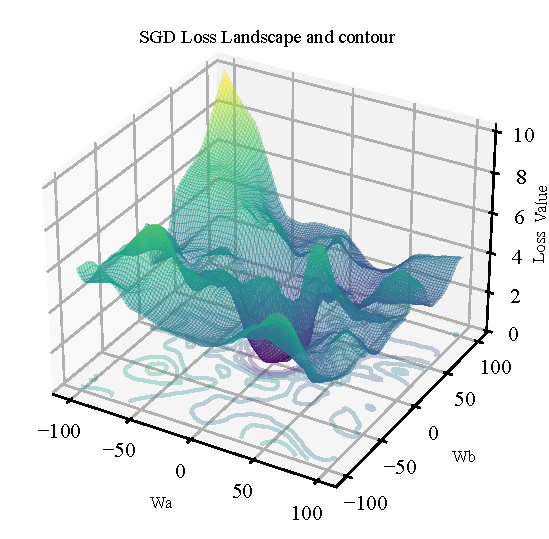
\includegraphics[width=\columnwidth]{images/SGD_LLC.pdf}
	\caption{Loss landscape and contour of SGD}
	\label{fig:SGD_LLC}
\end{figure}

With respect to the loss landscape as shown in \Cref{fig:SGD_LLC}, which generated based on the loss landscape work \cite{li2018visualizinglosslandscapeneural}. 
In the light of \Cref{fig:SGDvsPUGD} and the ideas that "flat" minimizers that generalize well \cite{chaudhari2017entropysgdbiasinggradientdescent}. Based on the explorations from Li et al.\cite{li2018visualizinglosslandscapeneural} and Jastrzebski et al.\cite{jastrzebski2020breakevenpointoptimizationtrajectories}. The training process can be illustrated as optimizer generally navigates the loss landscape by starting at random initial weights, iteratively moving opposite to noisy mini-batch gradients (which help escape saddle points), oscillating in narrow valleys due to high curvature, and eventually converging toward flat regions (minima) as the learning rate decays—behaving like a marble rolling down a bumpy slope with stochastic nudges. 
This motivates a two-way exploration into how perturbation radii (large vs. small) interact with training phases (early vs. late) — an underexplored dimension that may reveal optimal noise scheduling strategies. To explain it explicitly, The one is considered as (1) early training benefits from larger perturbation radii to escape poor initializations (e.g., saddle points in high-curvature regions), while later stages require smaller radii to fine-tune within flat minima basins. The another is (2) early training benefits from smaller perturbation radii to reach flat minimizers efficiently, while later stages require larger radii to expand the area of flat basins. These two approaches declared the background philosophy as whether to prioritize global exploration in early training (escaping poor initializations) or late training (expanding flat basins), constituting a continuum of noise-driven optimization strategies. Therefore, four tuning strategies were proposed in \ref{subsec:3.5}, by which multiply the $\epsilon_{t} (the unit perturbation)$ with an adaptive variable $\alpha$ to tuning the perturbation radius.

\subsection{Timing of application for PUGD}
\label{subsec:3.3}
Given that (a) perturbation may provide negligible benefits during early training stages (as hypothesized in \ref{subsec:3.2}), and (b) SGD and PUGD exhibit nearly identical performance in initial phases \Cref{fig:SGDvsPUGD}, we propose a phase-aware switching mechanism to dynamically activate PUGD only when its gradient modification proves statistically meaningful. Adapting the methodologies of Maclaurin et al. \cite{maclaurin2015earlystoppingnonparametricvariational} that stop training early based on specific criterion, two statistically-grounded ideas were proposed for adaptive optimization control: Dynamic triggering conditions based on 1. gradient statistics, 2. generalization gap
Derived from these two ideas, there are two methods to measure when to use PUGD as:
\begin{enumerate}
    \item[(1)] Gradient variance threshold: Calculate the variance of the L2 norm the current batch gradient: $\sigma ^{2} = Var(\left \|g_{t} \right \|_{2})$ (Sliding window statistics, such as past k=10 batches).
	Trigger condition: $\sigma ^{2} < \gamma \cdot  \sigma ^{2}_{init}$, $\sigma ^{2}_{init}$ is the mean gradient variance in the first k steps of training, $\gamma$ is attenuation coefficient (such as 0.2).
	\item[(3)] generalization gap monitoring: Calculate the generalization gap of resampling every T (like 3) epoch: $ \Delta = \left | L_{val} - L_{train} \right |$.
	Trigger condition: $\Delta > \mu \cdot \Delta _{base}$, $\Delta _{base}$ is initial gap, $\mu$ is proportional threshold (such as 2.0), $\Delta _{base} = \frac{1}{\xi} \sum_{i=1}^{\xi} \Delta _{i}$, which is the mean gap during the initial $\xi$ epochs. 
\end{enumerate}

The difference between fine tune pretrained model and the timing idea is that the proposed methods starting from random initialization and activate PUGD only when the triggering conditions are met. These dynamic strategies can be possibly adapted for fine-tuning scenarios, for example, model was already pretrained with optimizer A, then fine-tune with optimizers B and C.

\subsection{Scale of gradient Tunning}
\label{subsec:3.4}
This section introduces a method for tuning the scale of $g_t = \bigtriangledown f (w_t)$ (gradient of the loss function at t) when compared with $g_{t^{*}}$ (gradient from the unit perturbation $\epsilon_{t}$). As shown in \eqref{eq:3}, PUGD enforces a fixed ratio of 1 between these gradients, whereas SAM implicitly treats this ratio as 1:0. Empirical results from Tseng et al. \cite{4308316} demonstrate that PUGD outperforms SAM, suggesting that aggregating the original gradient and perturbation gradient (i.e., $g_{t^{*}} + g_t$) is empirically effective. This observation raises a critical question: What is the theoretically justified ratio between these gradients? Foret et al. \cite{foret2021sharpnessawareminimizationefficientlyimproving} proved that gradient descent via perturbation gradients can simultaneously suppress $g_t$ and sharpness. However, PUGD amplifies gradient effects through simple summation. The optimality of the ratio 1 remains uncertain—it may be a theoretically justified value or merely a heuristic choice. From a theoretical perspective, it remains ambiguous whether applying larger scaling factors to $g_t$ during early or late training stages would enhance generalization performance. The fundamental challenge lies in the lack of conclusive evidence about the correlation between gradient magnitude at specific training phases and final model robustness. Inspired by the considerations from tuning the perturbation radius \ref{subsec:3.2}, we propose to dynamically rescale the gradient $g_t$ during training through an adaptive parameter $\alpha$, employing tuning strategies \ref{subsec:3.5} similar to those used for perturbation radius adjustment. This approach enhances the contribution of $g_t$ to gradient updates and reveals phase-dependent scaling laws that govern the tripartite relationship between training phases, generalization performance, and scale of $g_t$.

\subsection{Four tuning strategies with $\alpha$}
\label{subsec:3.5}
Adapting the cosine annealing paradigm proposed by Loshchilov and Hutter \cite{loshchilov2017sgdrstochasticgradientdescent}, we implemented and compared four distinct tuning strategies during model training to evaluate their relative performance. The proposed algorithms and corresponding conceptual diagrams are illustrated as follows:
\begin{enumerate}
    \item[(1)] cosine annealing: 
	\[\alpha = \beta_{min} + (\beta_{max}-\beta_{min})\cos(\frac{\pi t}{2T})\]
    \item[(2)] inverse sine annealing: 
	\[\alpha = \left[\beta_{min} + (\beta_{max}-\beta_{min})\sin(\frac{\pi t}{2T})\right]^{-1}\]
    \item[(3)] sine heating: 
	\[\alpha = \beta_{min} + (\beta_{max}-\beta_{min})\sin(\frac{\pi t}{2T})\]
    \item[(4)] inverse cosine heating: 
	\[\alpha = \left[\beta_{min} + (\beta_{max}-\beta_{min})\cos(\frac{\pi t}{2T})\right]^{-1}\]
\end{enumerate}
Where T is the total num of epochs, t accounts for how many epochs have been performed since the last start. Max and min $\beta$ decide the uppper bound and lower bound of the $\alpha$. Heating contrasts with annealing, inducing monotonic increase in $\alpha$ during training. Inverse denotes the algorithmic inversion operation.

\begin{figure}[htbp]
	\center
	\vspace{-10pt} 
	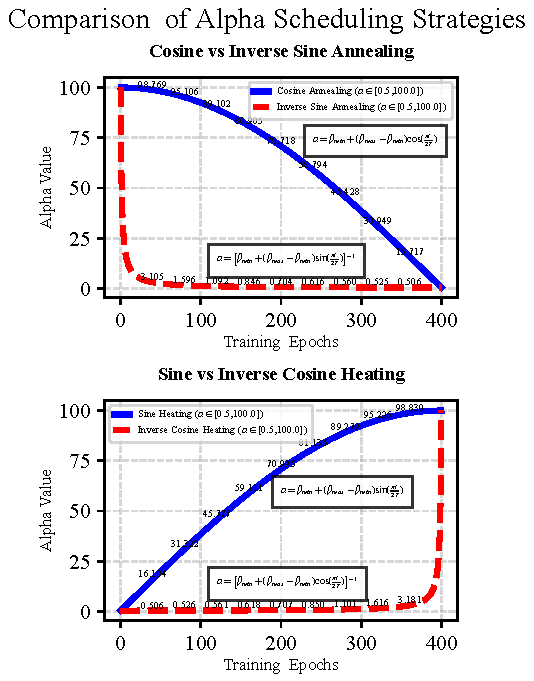
\includegraphics[width=\columnwidth]{images/AlphaSch.pdf}
	\caption{Comparison of alpha scheduling strategies
	\textbf{Top subfigure}: Cosine vs inverse sine annealing
    \textbf{Bottom subfigure}: Sine vs inverse cosine annealing
	The annotations are the decile-sampled values
	}
	\label{fig:AlphaSch}
\end{figure}

As illustrated in \Cref{fig:AlphaSch}, the main distinction between cosine annealing and inverse sine annealing lies in their decay dynamics: Cosine annealing exhibits a gradual decay of $\alpha$ throughout the training process. Inverse sine annealing rapidly decreases $\alpha$ during the initial 10\% of epochs (labeled with 3.105 in the figure), followed by a slower decay phase until converging to the minimum value $\beta_{min}$ (set to 0.5 in this example). Similarly, the main distinction between sine heating and inverse cosine heating lies in their growth dynamics: Sine heating exhibits a gradual growth of $\alpha$ throughout the training process. Inverse cosine heating increases $\alpha$ slowly during the last 90\% of epochs (labeled with 3.181 in the figure), followed by a rapid growth phase until converging to the maximum value $\beta_{min}$ (set to 100 in this example).

The benefits of inversion lie in the rapid adjustment of $\alpha$ (used for tuning both perturbation radius and gradient scale) during specific training phases. This dynamic behavior aligns more closely with the loss variation patterns observed in \Cref{fig:SGDvsPUGD} and \Cref{fig:SGD_LLC}, suggesting that abrupt changes—rather than gradual ones—may better capture underlying optimization patterns. While empirical evidence for this hypothesis remains to be established (including whether $\alpha$ should be larger or smaller for perturbation radius and gradient scaling), I additionally propose testing cosine annealing and sine heating strategies to systematically investigate their effects on model generalization.

Scope Clarification: My objective is not to present universally optimal tuning strategies, as Gastpar et al. \cite{gastpar2023fantasticgeneralizationmeasures} theoretically proved, uniformly tight generalization bounds are unattainable in overparameterized regimes without distribution-dependent or algorithmic priors. Rather, I demonstrate that the four strategies remain effective under specific conditions for tuning the perturbation radius and scale of gradient.

%%%%%%%%%%%%%%%%%%%%%%%%%%%%%%%%%%%%%%%%
% experiments
%%%%%%%%%%%%%%%%%%%%%%%%%%%%%%%%%%%%%%%%

\section{Experiments}
\label{sec:4}

In this section, we implemented two experiments, including (1) optimizing behaviours comparison and (2) finetuning comparison. The experiments were implemented on open datasets in the equipment with GTX 1060 Mobile, 6G Gpu RAM, and an i5-8400 CPU processor. Then were implemented on open datasets in the equipment with GTX 5090 Mobile,

In addition, every experiment followed the hyperparameters setting in the learning rate (LR)	= 0.1, weight decay = 0.0005, momentum = 0.9, Nesterov = False, and the learning schedule of cosine annealing \cite{loshchilov2017sgdrstochasticgradientdescent}. Every subject followed the same Pytorch 
default initial weights policy, a random uniform distribution with seed = 42. 

\subsection{Comparative analysis of optimization strategies for the CIFAR-10 dataset}
\label{subsec:4.1}

To observe the behaviours of PUGD with different strategies, this subsection of simulation has been organized into 3-folds:  
1. Perturbation radius Tuning, 2. Timing of application, 3. Scale of gradient Tunning. Through these observations, we can get a picture of what these strategies can do 
with models. 

\subsubsection{Perturbation radius Tuning}
\label{subsec:4.1.1}

\begin{figure}[htbp]
	\center
	\vspace{-10pt} 
	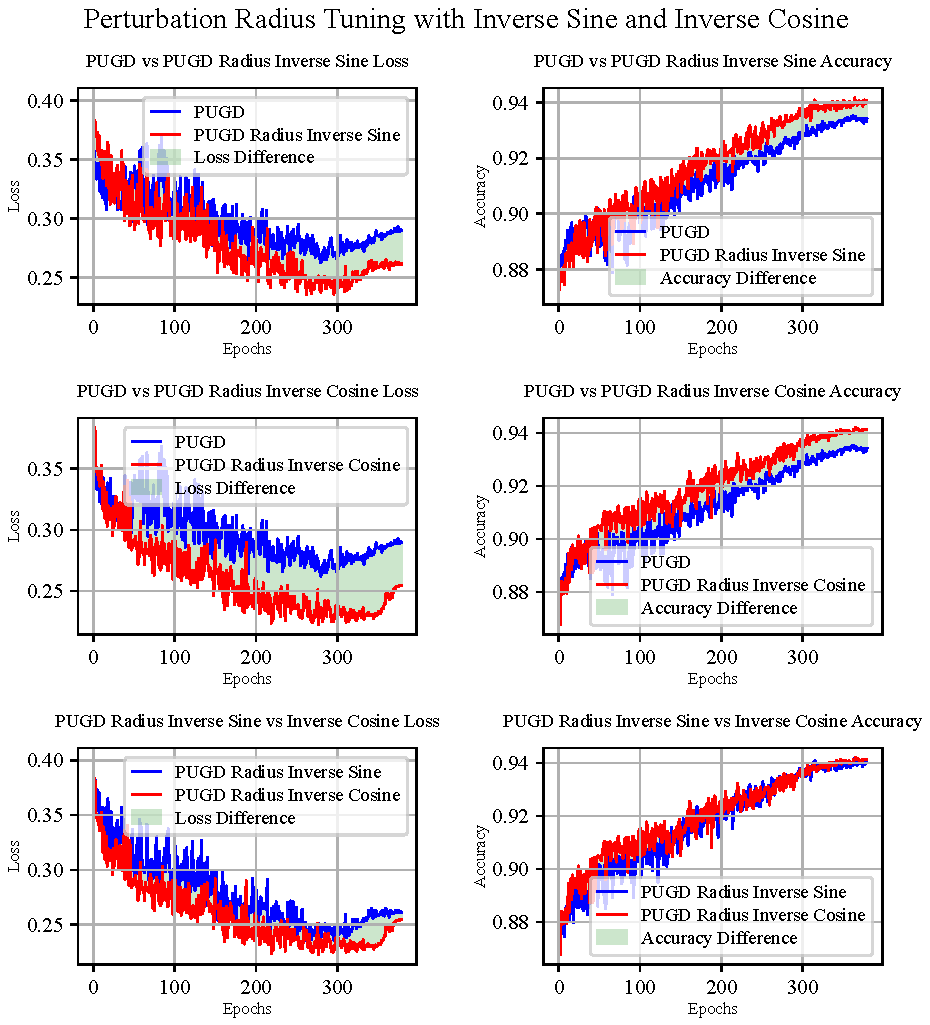
\includegraphics[width=\columnwidth]{images/PUGDRadiusInv.pdf}
	\caption{Perturbation Radius Tuning with Inverse Sine and Inverse Cosine
	\textbf{Top left (a)}: Pugd vs Pugd Radius inverse sine loss \textbf{Top right (b)}: Pugd vs Pugd Radius inverse sine accuracy
    \textbf{Middle left (c)}: Pugd vs Pugd Radius inverse cosine loss \textbf{Middle right (d)}: Pugd vs Pugd Radius inverse cosine accuracy
	\textbf{Bottom left (e)}: Pugd Radius inverse sine vs inverse cosine loss \textbf{Bottom right (f)}: Pugd Radius inverse sine vs inverse cosine accuracy
	The epochs ranged from 21 to 400, $\beta_{min}$ set as 0.01 and $\beta_{max}$ set as 2 for both inverse sine and cosine.
	}
	\label{fig:PUGDRadiusInv}
\end{figure}

As shown in \cref{fig:PUGDRadiusInv}, both strategies (inverse sine and cosine) consistently outperformed native PUGD. Although the best accuracy improvements were marginal (0.9353 vs. 0.9419/0.9417), two critical patterns emerged:  
\begin{itemize}
    \item The performance gap \textit{w.r.t} PUGD widened progressively with more epochs, evidenced by growing differences in both loss and accuracy metrics  (subfigure a, b, c, d).
    \item Between the two strategies, inverse cosine demonstrated superior loss minimization despite nearly identical accuracy trajectories (subfigure e, f).
\end{itemize}
Unfortunately, the experimental results only demonstrate that both strategies can optimize model performance beyond the baseline achieved by the native PUGD method. However, they cannot substantiate the theoretical assumptions proposed in \cref{subsec:3.2}, since the two strategies produced statistically equivalent results. This equivalence suggests that the futher investigation needed.


One additional thing has to be noticed is that loss was increased during the accuracy increase after 300 epochs, which was explained by Ishida et al. \cite{ishida2021needzerotrainingloss} as the "overfitting" problem. The reason is overfitting or inconsistent distribution of training validation data, that is, in the later stage of training, the predicted results tend to be extreme, causing a small number of incorrectly predicted samples to dominate the loss, but at the same time, a small number of samples do not affect the overall validation accuracy. Due to the time limitation and the fact that the benchmark (native PUGD) didn't solve this problem, this study is unable to address this issue either.. For subsequent researchers or developers, if you want to overcome this problem, you can try (1) Increase training samples, (2) Increase the weight of regularization coefficients, (3) Add early stopping mechanism \cite{bai2021understandingimprovingearlystopping}, (4) Adopting Focal Loss \cite{lin2018focallossdenseobject}, (5) use Label Smoothing \cite{szegedy2015rethinkinginceptionarchitecturecomputer}

Note: The training curves of the initial 20 epochs were excluded from visualization due to their statistically indistinguishable patterns.

\begin{figure}[htbp]
	\center
	\vspace{-10pt} 
	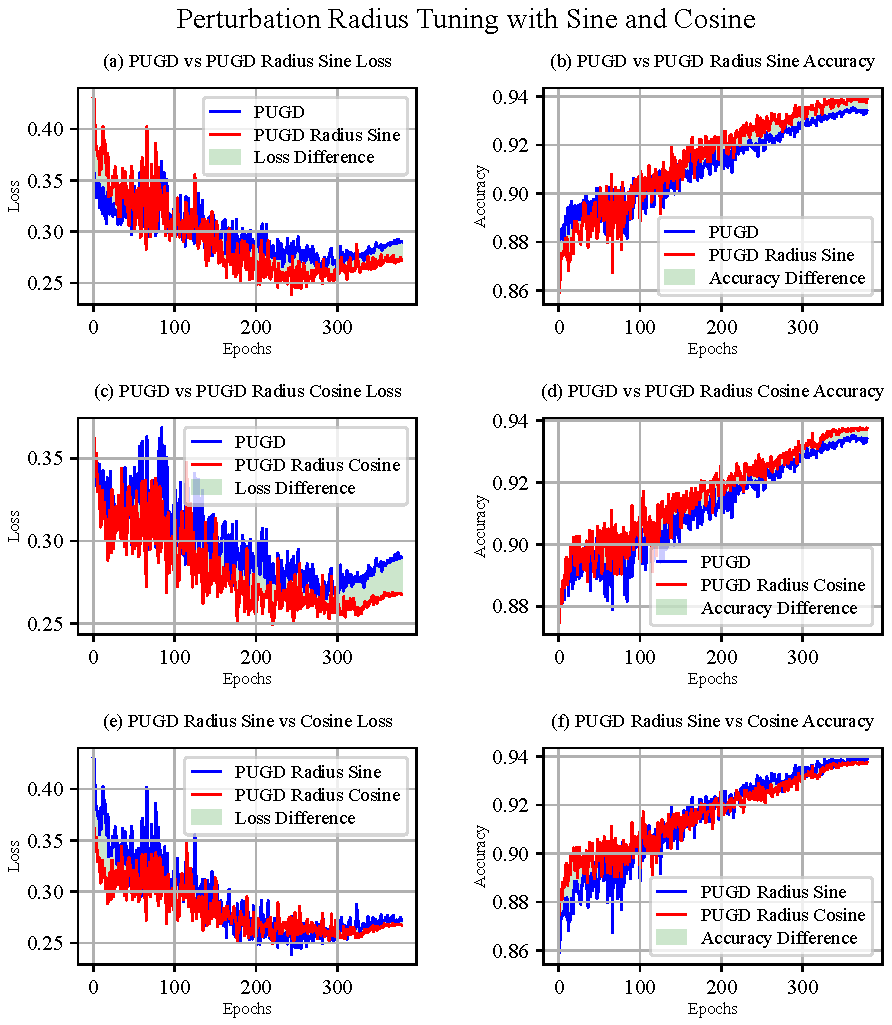
\includegraphics[width=\columnwidth]{images/PUGDRadius.pdf}
	\caption{Perturbation Radius Tuning with Sine and Cosine
	\textbf{Top left (a)}: Pugd vs Pugd Radius sine loss \textbf{Top right (b)}: Pugd vs Pugd Radius sine accuracy
    \textbf{Middle left (c)}: Pugd vs Pugd Radius cosine loss \textbf{Middle right (d)}: Pugd vs Pugd Radius cosine accuracy
	\textbf{Bottom left (e)}: Pugd Radius sine vs cosine loss \textbf{Bottom right (f)}: Pugd Radius sine vs cosine accuracy
	The epochs ranged from 21 to 400, cosine used $\beta_{min}$ as 0 and $\beta_{max}$ as 1, sine used $\beta_{min}$ as 0 and $\beta_{max}$ as 2.
	}
	\label{fig:PUGDRadius}
\end{figure}

As shown in \cref{fig:PUGDRadius}, (a) and (b) showed that 



\subsubsection{Timing of application}
\label{subsec:4.1.2}

\subsubsection{Scale of gradient Tunning}
\label{subsec:4.1.3}

\begin{figure}[htbp]
	\center
	\vspace{-10pt} 
	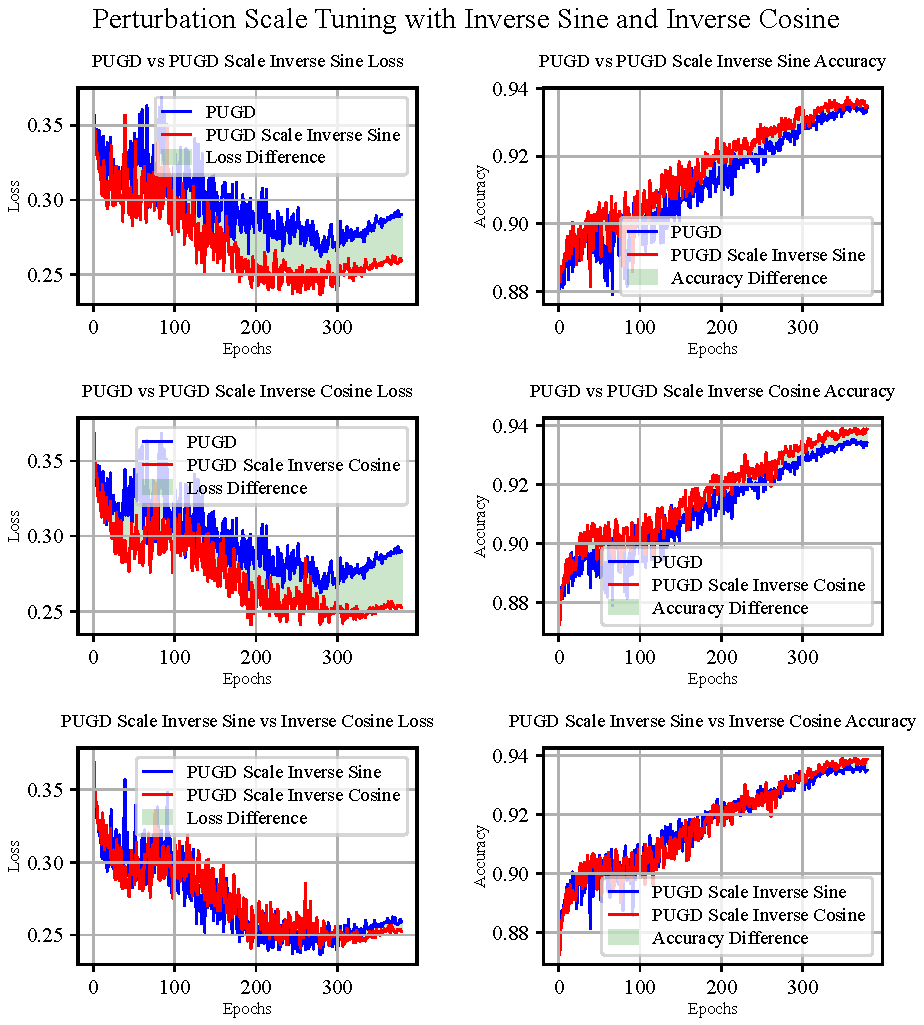
\includegraphics[width=\columnwidth]{images/PUGDScaleInv.pdf}
	\caption{Perturbation Scale Tuning with Inverse Sine and Inverse Cosine
	\textbf{Top left (a)}: Pugd vs Pugd Scale inverse sine loss \textbf{Top right (b)}: Pugd vs Pugd Scale inverse sine accuracy
    \textbf{Middle left (c)}: Pugd vs Pugd Scale inverse cosine loss \textbf{Middle right (d)}: Pugd vs Pugd Scale inverse cosine accuracy
	\textbf{Bottom left (e)}: Pugd Scale inverse sine vs inverse cosine loss \textbf{Bottom right (f)}: Pugd Scale inverse sine vs inverse cosine accuracy
	The epochs ranged from 21 to 400, inverse cosine used $\beta_{min}$ as 1 and $\beta_{max}$ as 2, inverse sine used $\beta_{min}$ as 0.8 and $\beta_{max}$ as 3.
	}
	\label{fig:PUGDScaleInv}
\end{figure}




\subsection{Radius-Timing Scale(RTS)}
\label{subsec:4.2}

\subsection{Finetuning comparison}
\label{subsec:4.3}





%%%%%%%%%%%%%%%%%%%%%%%%%%%%%%%%%%%%%%%%
% conclusions
%%%%%%%%%%%%%%%%%%%%%%%%%%%%%%%%%%%%%%%%

\section{Conclusions}
\label{sec:5}
This article didn't aims to provide the best parameters, but to provide the enhancement methods RTS 







%%%%%%%%%%%%%%%%%%%%%%%%%%%%%%%%%%%%%%%%
% bibliography
%%%%%%%%%%%%%%%%%%%%%%%%%%%%%%%%%%%%%%%%

{\small
\bibliographystyle{ieee_fullname}
\bibliography{main}
}

\end{document}



\newpage
\appendix
\section{Appendix}
\label{appendix}
\subsection{Comparative analysis of optimization strategies for the CIFAR-100 dataset}
\label{appendix:cifar100}
\begin{table}
	\begin{center}
		\begin{tabular}{|l|c|c|c|c|}
			\hline
			Methods & $\beta_{min}$ & $\beta_{max}$ & Best Accuracy \\
			\hline
			PUGD	& None &	& None & \bf{0.7188} \\
			\hline
			Radius inverse cosine &  &	&  & \bf{} \\
			Radius inverse sine 	& 0.01 &	& 2 & \bf{0.7315} \\
			Radius cosine &  &	&  & \bf{} \\
			Radius sine 	& 0.0 &	& 1.0 & \bf{0.7199} \\
			\hline
			Scale inverse cosine & 0.8 &	& 3 & \bf{0.7222000000000001} \\
			Scale inverse sine 	& 0.1 &	& 2 & \bf{0.7267} \\
			Scale cosine & 0.0 &	& 1.0 & \bf{0.7209} \\
			Scale sine 	&  &	&  & \bf{} \\
			\hline
		\end{tabular}
	\end{center}
	\caption{%
		The best accuracy of different strategies for Radius and Scale Tunning
	}
	\label{tab:cifar100}
\end{table}

